\chapter{Introduction}
\label{sec:intro}

\section{Motivation}
\label{sec:motivation}
Route queries present an important class of spatial queries for users to request an efficient path by specifying a source and a destination. A \textit{Sequenced Route Query} (SRQ) is defined as finding the shortest path from a starting point towards a possible destination, passing through multiple locations, defined by their category type (introduced as Category of Interest (CoI) in this thesis). As an essential component, this type of route queries are widely supported by many of today's online map service providers (e.g., Google Maps, Yahoo! Maps, Bing Maps etc). There has been significant research and proposed approaches on the topic of sequenced route queries, but there has not been developed a query language to provide more flexibility to these types of queries. The work in this thesis has been focused on researching the topic of sequenced route queries in road networks and designing a language to enable the user to express his requirements in the form of a user query in a flexible manner, such as applying different constraints and rules on the route to be found.

\textbf{Example:}

Figure \ref{fig:example} presents a small example network with four different CoI sets, illustrated with different colors. The colored circles represent the Points of Interest (PoIs) and the lines between them represent the roads, whereas every road is associated with a weight corresponding to its length. In total there is two restaurants, a movie theater, two banks and two pharmacies. The starting point \textit{sp} is represented by a rhombus.

Suppose that a user is planning a trip to town: he first wants to go to a restaurant for lunch, then he wants to stop by a bank, then he meets a friend in the movie theater and after that he plans to have a dinner at a restaurant. In this specific scenario, the user wants to express his wish for both restaurants to be the same, because he may prefer a route where the equality of the two restaurant PoIs is more important to him than the length of the route itself.

With existing approaches, the user can get the shortest route \cite{OSR} approach or all routes that satisfy the semantic similarity and length conditions equally \cite{semanticSRQ}, but that does not guarantee the equality of the two restaurant PoIs. Also finding \textit{k} number of optimal routes, which answering the user's SRQ and then filtering out the routes where the two PoIs of type restaurant are equal has proven to not always generate a result, which is why in this thesis a better optimal approach is presented.

\enlargethispage*{30pt}

Using Figure \ref{fig:example}, we see that the user query in the example above, when answered as an \textit{Optimal Sequenced Route} (OSR) query \cite{OSR}, delivers the route $(r_1, b_1, mt_1, r_2)$ with length 11 (shown with red lines in the figure), where both restaurants $r_1$ and $r_2$ are different. Our proposed approach, on the other hand, strives to find the optimal route, where the two restaurants are equal. The delivered route will not necessarily be the shortest possible sequenced route, but it will be the shortest route out of all possible routes, where the two PoIs are equal to each other. Such route in our example graph would be $(r_1, b_1, mt_1, r_1)$ with length 12 (shown with dashed lines in the figure).

Specific constrains such as the equality in this example are proposed in the thesis as operators on the query. We modified and extended existing approaches, which answer the Optimal Sequenced Route (OSR) Query such as the \textit{Progressive Neighbor Exploration} (PNE), proposed in \cite{OSR}, in order to transform the complex user query and retrieve desired results.

\begin{figure}[H]
	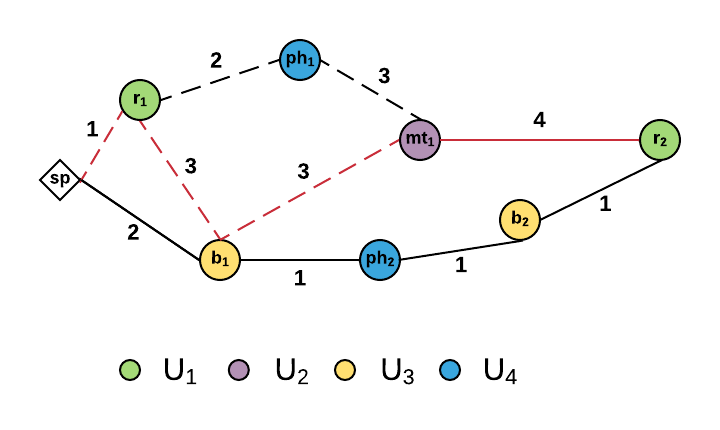
\includegraphics[scale=1]{images/Example_routes.png}
	\centering
	\caption{A network with four different types of point sets}
	\label{fig:example}
\end{figure}

\section{Problem definition}

With the rise of location based mobile services the need for a query language to answer complex route queries has emerged. To the best of our knowledge, although different approaches to answer the sequenced route query have been proposed, no one has yet identified the need for a unified query language to answer this complex route query types. What we would like to achieve with this thesis is to identify the problem, which is the need for flexibility in terms of route queries, and to propose a comprehensive solution to the problem. Through scientific research and research on the user's specific needs in this area of route queries, we have come up with several important operators that should be a part of this query language. Since the query language is entirely based on the user's requirements, which include individual personal needs, the query language operators that we propose are not a complete set. We propose four operators, that we deem the most important in terms of the level of flexibility they give to the user, and give an outlook on other ones, which can enrich the language in the future. \newline
One of the most important comparison operators in programming and query languages is the equality operator. Therefore we decided to develop an articulate version of the equality operator for the route query type, and also developed the opposite not-equality operator in addition. Another very important programming and database language operator is the logical or operator, which gives the user the flexibility to define a subset of possible query variants that have to be filtered to obtain the best result. And lastly, we propose the order operator, which transforms the \textit{sequenced} route query in a \textit{partially sequenced} or \textit{not sequenced} route query. This type of operator is closely related to the \textit{Traveling Salesman Problem (TSP)}, which asks for the sequence in which a set of given points from a starting point is visited. The reason for choosing to design this operator is the strive for maximum flexibility. In this respect, the order operator represents the highest level of flexibility when it comes to planning a trip as a tourist with the intention of visiting multiple locations in a short period of time, without much need for order of the different types of locations.

% e.g. performance, processing time for the trivial approach 
\section{Challenges}
When working with real-life road networks, we are usually posed with the challenge of having big datasets with many PoIs. This makes it difficult to design fast algorithms for route finding queries without the need for optimizations techniques. Trivial approaches usually explore the entire search space in order to find one optimal solution, which especially in the case of route queries can increase the time exponentially. If we need to check all neighbors to one PoIs of one category and do this for all categories in order to find the shortest route from a category sequence, the time in the case of the trivial approaches increases exponentially with increase in the size of the category sequence. The \textit{Optimal Sequenced Route Query} \cite{OSR} presents the PNE approach, which solves the OSR query in metric spaces efficiently. The challenge for our task is to be able to use this designed approach to implement the proposed operators. \newline
As shown in the example in Section \ref{sec:motivation} the Progressive Neighbor Exploration (PNE) approach doesn't always address user's requirements, therefore we need to modify the algorithm to serve our needs. In order to make sure that the algorithm delivers an optimal result, all routes must be checked, where two specific PoIs of one category are equal. This means that all PoIs of this category must be somehow inspected, which increases the search space significantly, which in turn spikes the processing time of the query. This poses the need for an optimization technique, such as the heuristic approach, presented in Chapter \ref{ch:EO}, to shrink the search space. \newline
The requirement for not-equality, translated as the need for two PoIs of the same category to be different, is also not always addressed by the PNE approach. As in the example above, the shortest route may be one, where the two PoIs are the same. Therefore, in order to take this requirement into account we develop an optimal algorithm to answer this type of query. We call this the not-equality operator. \newline
Furthermore, the or operator and the order operator are faced with the challenge for exponentially growing permutations, depending on the size of the query. Therefore the trivial approaches, which simply build all possible permutations of the query and perform the PNE approach on them, can generate a big search space and increase the time exponentially with the increase in the number of permutations. In our proposed approaches for these two operators we build an optimal algorithm, which is able to work on the possible permutations simultaneously, while pruning longer routes, which may be generated when the permutations are handled separately. In this way we shrink the search space, while also making sure that the algorithm does not prune suitable candidates without examining them.

% Shortly presenting the algorithms for the operators; experiment results, comparing to the baseline approach
\section{Contributions}
In this thesis, we introduce four different operators, which can be applied to a route query, and propose alternative approaches for solving them, which outperform the trivial solutions. We developed optimal algorithms which take the user's requirements into account and find the optimal solutions efficiently. The presented algorithms relate to the following operators: equality operator (EO), not-equality operator (NEO), or operator (OR) and order operator (ORDER). The equality operator addresses the need for flexibility, introduced in the example in Section \ref{sec:motivation}, and the not-equality solves the opposite problem, in which the user specifically wants two different PoIs of the same category type in the query. Furthermore, the or operator represents the disjunction operator, usually present in query languages, and it gives the user the possibility to apply multiple category options to one or more route query points. Lastly, the order operator provides the user with the option to have a partially or fully not sequenced route query, where he can define zero or multiple categories to be at fixed positions in the route query sequence. \newline
The algorithms for solving the operators are inspired by the PNE approach, presented in the \textit{Optimal Sequenced Route Query} \cite{OSR}. For answering the equality operator query, a heuristic approach is explored, as well, for shrinking the search space and reducing the processing time. For the three of the operators (EO, OR and ORDER) baseline approaches are also introduced and compared to the proposed approaches in the experiment results. Our introduced algorithms outperform the trivial solutions in the experiments with a real dataset significantly, especially with increasing the search space with the help of different evaluation parameters, which further shows the efficiency of our proposed algorithms.

\section{Outline}
The remainder of the thesis is organized as follows: First, in Section \ref{sec:notes} we introduce the notations used in the thesis, then we review the related work that has been done on the topic of SRQ in Section \ref{sec:relwork}. In Section \ref{sec:operators} we cover the proposed operators and go into details on some of them in separate sections for each of them: Motivation, Problem definition and Proposed approach. In Section \ref{sec:evaluation} we present the results from the experimental studies, performed on the implemented operators and we evaluate the results. Finally, in Chapter \ref{sec:conclusion} we conclude the thesis by summing up the progress made on the subject and discuss future work.